Nyní je tedy na čase\todo{radši bych tyto části psal víc formálně... Na základě provedené analýzy je možné... (i u ostatních částí)} připravit návrh řešení aplikace, která by zajistila správu modulárních dokumentů, jejich generování/publikaci. Nesmíme zapomenout
na důležité funkcionality, které jsme si stanovili v první části této kapitoly. Jedná se hlavně o správu uživatelů, možnost tvořit revize a celkově
verzovat jednotlivé části textu. Dále nesmíme zapomenout na možnost rozšíření aplikace.

\section{Užitelská sekce}

V uživatelské sekci bude hlavní důraz kladen na správu uživatelů, zde také musíme myslet na ochranu jejich osobních udajů a díky GDPR také na
možnost jejich anonymizace. Také je potřeba brát v úvahu rozdělení uživatelů na standardní a administrátorské role, které mají rozdílné oprávnění.
Uživatelem se stává osoba při první interakci s aplikací, v tuto chvíli je osoba brána pouze jako host. Aby se uživatel stal plnohodnotným uživatelem,
je třeba se nejdříve registrovat, tím si užvatel\todo{ouch} vytvoří vlastní uživatelský účet, který bude mít standarní\todo{ouch} práva. Pro získání administrátorských
oprávnění je potřeba jiného administrátora, který může běžný účet prohlásit za administrátorský. Ještě bude existovat uživatel se oprávněním
\uv{super admin}, který bude mít práva na všechny operace v rámci systému.

V rámci zjednodušení práce s právy na jednotlivých dokumentech a repozitářích, o kterých se zmíníme později v této kapitole, zavedeme uživatelsky
definované role, které bude poté možné přiřazovat všem uživatelům. Tyto role budou sloužit k hromadným operacím na uživateli, toto ovšem bude
přístupné pouze uživatelům, kteří budou mít roli administrátora.

\subsection{GDPR}
\todo{GDPR}
\subsection{Příklady užití}

\section{Repozitáře}

\todo{Na tohle by se hodil nějaký obrázek/diagram}
Než začneme popisovat samotné generování dokumentů, je potřeba si definovat repozitáře našich modulů. Jednotlivé repozitáře nám budou sloužit jako složky,
které budou obsahovat moduly, ze kterých se pak budou skládat výsledné dokumenty. V rámci repozitářů je potřeba hlavně zajistit správně fungování oprávnění.
Pokud si uživatel založí nový repozitář, má vůči němu všechny práva, ostatní uživatelé se o tomto repozitáři v tomto stavu nemají jak dozvědět, je pro ně
skrytý. Pokud se ovšem zakladatel rozhodne svůj obsah repozitáře sdílet, má možnost sdílet repozitář s jednotlivými uživateli, uživatelskými rolemi a nebo
změnit repozitář na veřejný. Dále má také možnost definovat, jestli je repozitář pro jednotlivé uživatele pouze pro čtení, či použití modulu v dokumenty,
nebo jestli je možnost moduly i upravovat.

V neposlední řadě musíme myslet na verzování našich jednotlivých modulů, zde se nabízejí 2 možnosti jak tomuto přistoupit, buď by bylo možné integrovat
řešení založené na nějaké vcs \todo[inline]{vysvětlit vcs}, nebo je možné implementovat verzování pomocí databáze. V této práci se vydáme cestou\todo{raději zase formálně ``je zvolena'', ``vybrána'', ...}
verzování pomocí databáze\todo{proč?}, to zařídíme

\subsection{Přehled všech příkladů užití}

\section{Dokumenty}

% this might be used, but not now
% \begin{center}
%     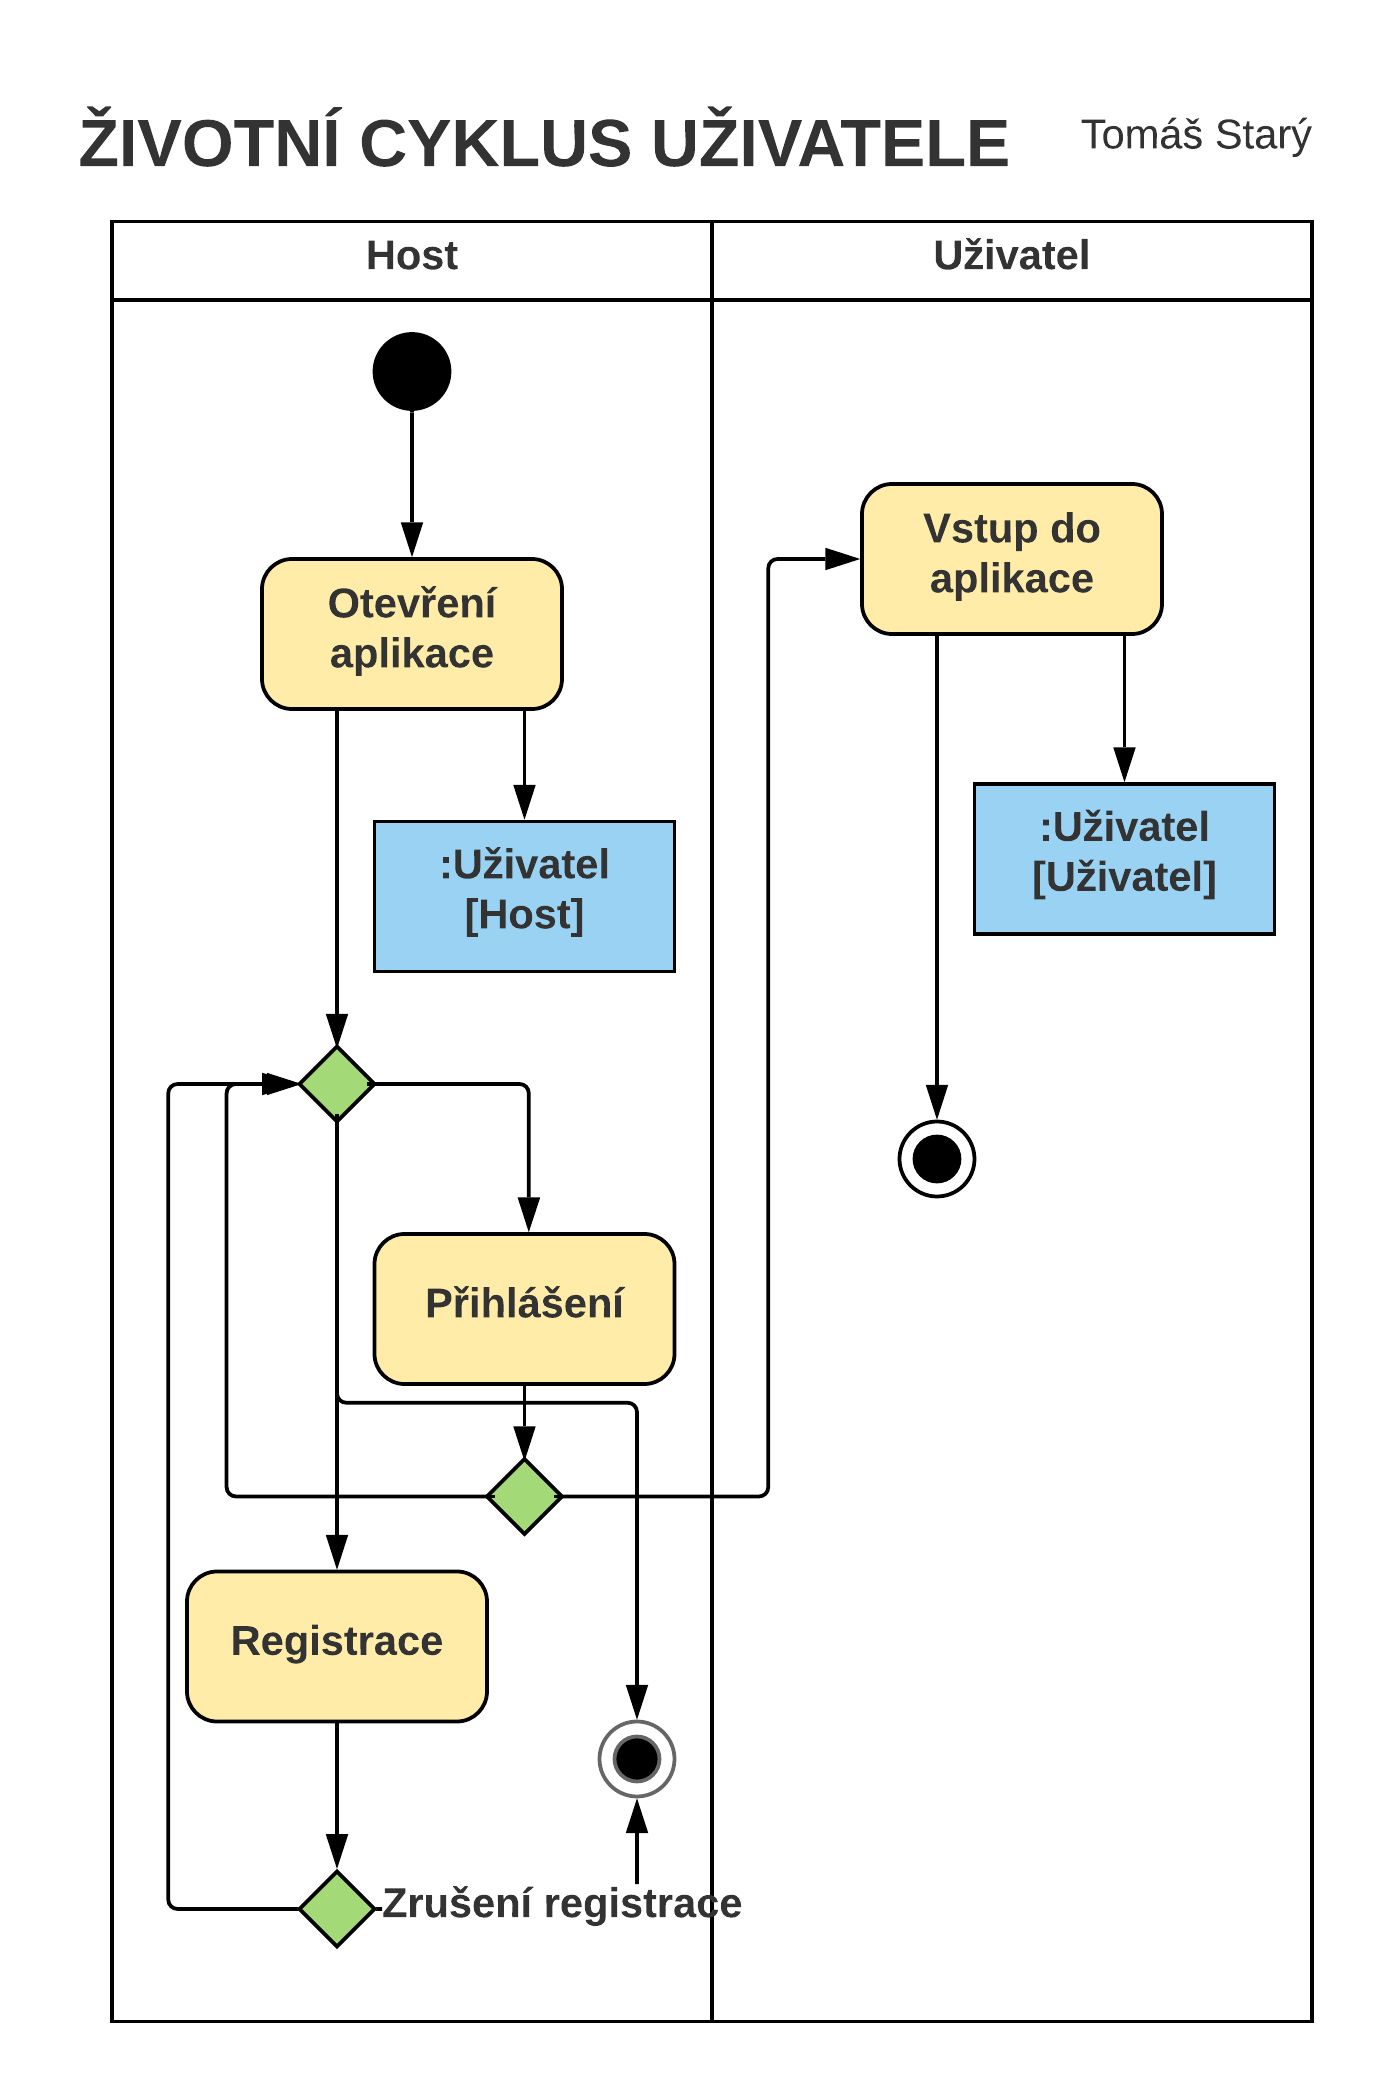
\includegraphics[width=8cm]{lifecycle.png}
% \end{center}